\section{shapes and fonts: examples}

\begin{figure}
	\centering
	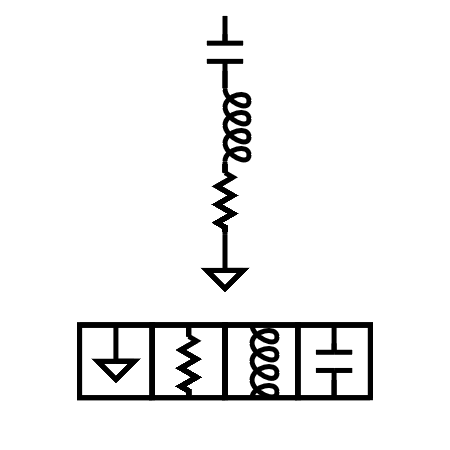
\includegraphics[width=4in]{figures/rlc.png}
	\caption[RLC]
	{RLC circuit.}
\end{figure}

\begin{figure}
	\centering
	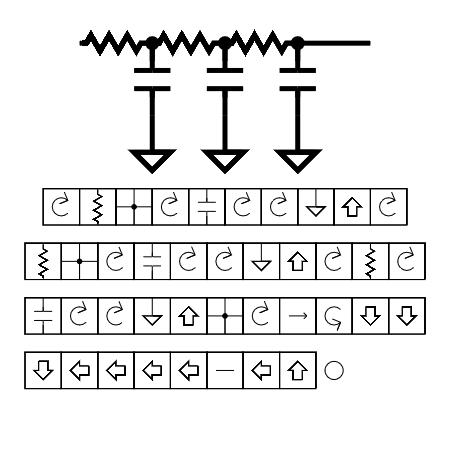
\includegraphics[width=4in]{figures/rcline.png}
	\caption[RCline]
	{RC line circuit.}
\end{figure}


\begin{figure}
	\centering
	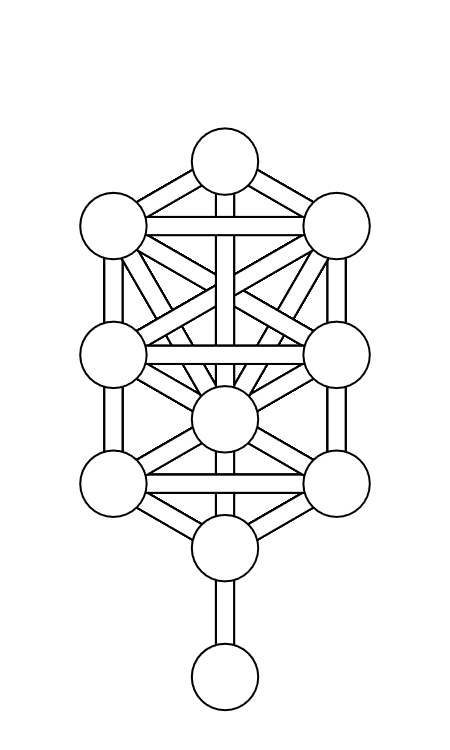
\includegraphics[width=4in]{figures/treeoflife.png}
	\caption[treeoflife]
	{The Tree of Life from Jewish mysticism.}
\end{figure}

\begin{figure}
	\centering
	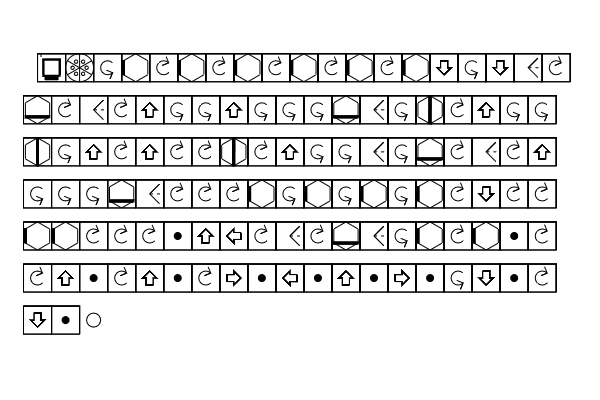
\includegraphics[width=4in]{figures/treeoflifespelling.png}
	\caption[treeoflifespelling]
	{Symbol glyph spelling of Tree of Life. What makes things like this easy to make is building up building blocks like the cross pieces of all different scales, and the use of universal symmetries and scales(6 fold, 12 fold, and the square root of 3 and 2).}
\end{figure}




\begin{itemize}
\tightlist
\item
editing shape stack, workflow, how to share, upload, download, send and store, same with fonts, connect to hypercube
\item
basic shapes built into 0200 thru 0217, how it's all connected to 01xxx
\item
pixel fonts
\item
laser cut fonts
\item
signal flag font
\item
general circuits
\item
quantum circuits
\item
graph theory, with digression into how to operate Maps with mathjax formatting for fully tex compatible graph theory figure creation
\item
quantum logic gates
\item 
classical logic gates
\item
standardized icon design for geometron system
\item
katakana
\item
hebrew
\item
laser cut shape set shape stack
\item
laser cut ruler
\item
laser cut protractor
\item
tree of life from western occult practice
\item
penrose tiles, fun with golden ratio, fivefold symmetry
\item
cross stitch design
\end{itemize}